\section{Software Development Life Cycle}
\label{sec:sdlc}

\ac{SDLC}\index{software development life cycle} is the fundamental process of software development that involves series of steps or phases, ensures the software completion.
Essentially speaking, it is a series of steps that provide a model for a or collection of software development and its lifecycle management.

\begin{figure}[htbp]
    \centering
    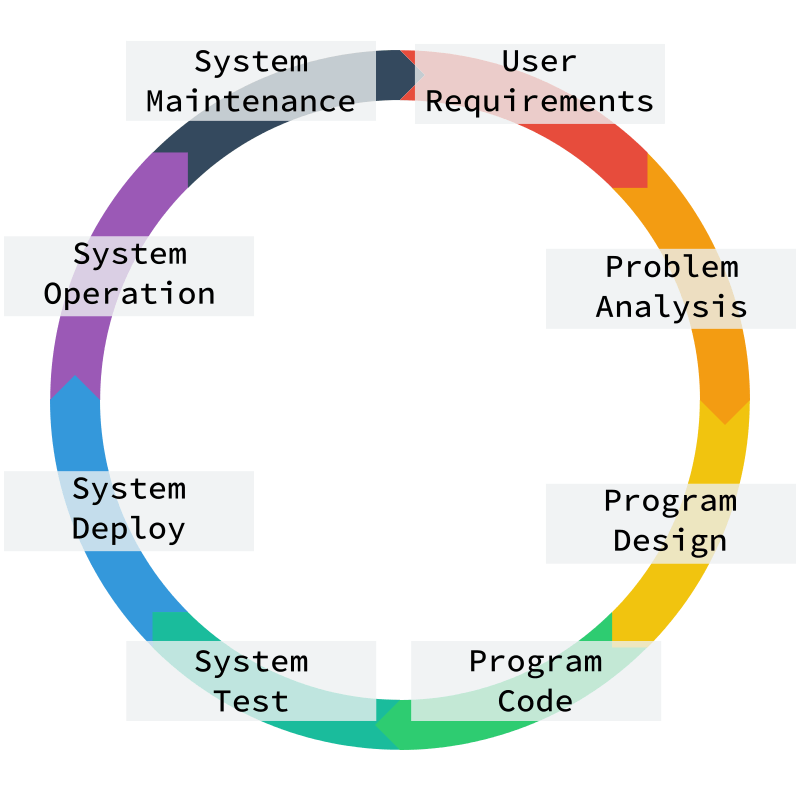
\includegraphics[width=0.8\textwidth]{\dir/include/sdlc.png}
    \caption{Common SDLC Cycle}
    \label{fig:sdlc:cycle}
\end{figure}

As in \autoref{fig:sdlc:cycle}, commonly there are step components like requirements, analysis, design, development (coding), test, deployment, operation, evaluation, and maintenance.
In this kind of traditional \ac{SDLC}, each step should finished its process before go into the next step.

% --------------------------------------------------
\subsection{Agile Methodologies}

Agile is a time boxed, iterative approach to software delivery that builds software incrementally from the start of the project, instead of trying to deliver it all at once near the end.
It works by breaking projects down into little bits of user functionality called user stories, prioritizing them, and then continuously delivering them in short two week cycles called iterations.~\autocite{Rasmusson2015Agile}
\autoref{fig:agile-a} and \autoref{fig:agile-b} shows how agile works in the process and iteration with a simple illustration.

\begin{figure}[htbp]
    \centering
    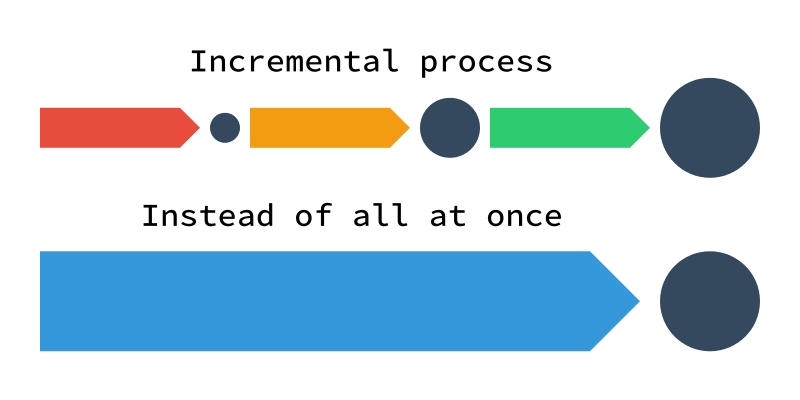
\includegraphics[width=8cm]{\dir/include/agile-a.png}
    \caption{Agile progress}
    \label{fig:agile-a}
\end{figure}

\begin{figure}[htbp]
    \centering
    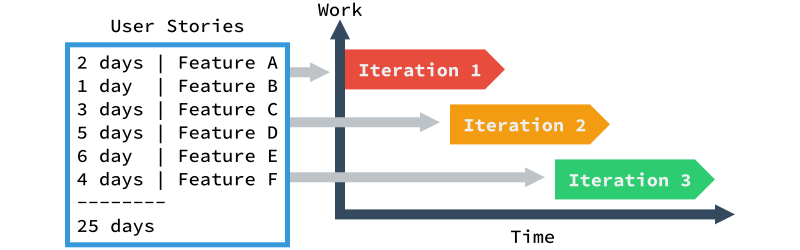
\includegraphics[width=12cm]{\dir/include/agile-b.png}
    \caption{Agile iteration}
    \label{fig:agile-b}
\end{figure}

Therefore, we don't risk in creating a big or even a thing that small for a long time.
Because we can frequently iterate the result, coming back again as like a improved beginning.
Essentially, we learn and relearn what we could have done in each iteration process.
In a process matter of sense, analysis, design, development/coding, and testing are continuous activities.
In addition, there are some key points that required and make agile considered to be greatly modern:

\begin{easylist}
& Development itself is iterative
& Planning is adaptive
& The scope variables may vary
& Requirements can change over time
& Working software is the primary measure of success
& Temporary or finished software can be done at all time
& Team members can be independent to each other, since there are cross-functional teams
& High cooperation can occur between technical and non-technical person
& and other leaned segments or aspects to consider
\end{easylist}

Agile is the counterpart of traditional \ac{SDLC}, and it is not just one thing, but a group of methodologies.
As in traditional \ac{SDLC} like waterfall approach, we cannot change easily any of its parts until it had complete its step.
So if a change is really needed, most likely the entire project will be build from the start again.
In agile for example, we can do fix and test at the end of each development step, depending on the corresponding step that matters.
Simply, agile methodologies provide flexibility to make changes, allow for any modification along the progress of \ac{SDLC}.
Hence there could be simultaneous development of different steps at the same time.
But back again, it would depend on the team's or personal's task distribution.
If the conditions are met, agile is more relevant to be used in real modern software development.

%Agile even has a manifesto that offer how convenience agile is, called \textit{Manifesto for Agile Software Development}~\autocite{Beck2001Manifesto}:

% --------------------------------------------------
\subsection{Minimum Viable Product}

Agile methodologies also heavily corresponds with building a \ac{MVP}\index{Minimum Viable Product} or we can also called it a \ac{MWT}\index{Minimum Working Thing}. Shortly defined, each elements of \ac{MVP} are~\autocite{Montgomery2013MWT}:

\begin{description}
  \item[Minimum] The least or smallest amount possible.
  \item[Viable] Capable of working successfully.
  \item[Product] An article or substance that is created or refined for sale.
\end{description}

Based on those elements, \ac{MVP} is a...
%TODO definition

\begin{figure}[htb]
    \centering
    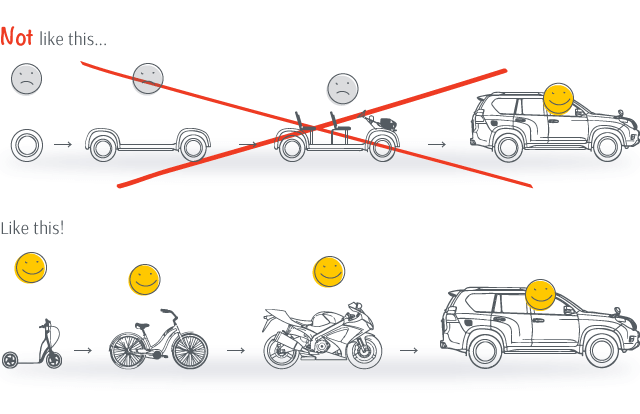
\includegraphics[width=\textwidth]{\dir/include/mvp-1}
    \caption[MVP illustrated]{MVP illustrated with only one usable product and some incremental products~\autocite{Mercury2014MVP}}
    \label{fig:method:mvp-1}
\end{figure}

We can also illustrate it as creating a vehicle with two different steps.
As in \autoref{fig:method:mvp-1}, the first one is a need to take a lot of steps of before finally finished the final usable product.
The second one is an incremental steps of creating the usable product, until it's final yet to be usable as visioned and planned.
It can be seen that the second approach is more appealing and effective than the first.

\begin{figure}[htb]
    \centering
    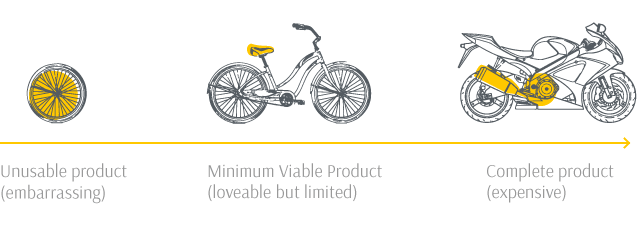
\includegraphics[width=\textwidth]{\dir/include/mvp-2}
    \caption[MVP compared]{MVP compared with unusable and complete product~\autocite{Mercury2014MVP}}
    \label{fig:method:mvp-2}
\end{figure}

Also as in \autoref{fig:method:mvp-2}, \ac{MVP} is compared with unusable product and complete product.
In this context, \ac{MVP} is ideally more balanced and preferable than the others.
More than that, if there is more effort and time, we can build a \ac{MLP}\index{Minimum Loveable Product}.
Which is an \ac{MVP} but taken beyond a working thing, which the customer will actually love using.
It's an embodiment of a production ready and could potentially get a customer or lots of them.
The thing that matters and can be used well.
Although it expected to be a real matter, such preliminary model like a protoype, a mockup, or even a set of data can sometimes considered as an \ac{MVP}.

% --------------------------------------------------
%\subsection{Extreme Programming}

%TODO illustration
%TODO Reason
%TODO About documentation

% --------------------------------------------------
\subsection{Testing with NAME}

%TODO Software or Design?

% The main reason

%TODO Reason

Black-box testing treats the software as a "black box", examining functionality without any knowledge of internal implementation. The testers are only aware of what the software is supposed to do, not how it does it.[23] Black-box testing methods include: equivalence partitioning, boundary value analysis, all-pairs testing, state transition tables, decision table testing, fuzz testing, model-based testing, use case testing, exploratory testing and specification-based testing.
